\documentclass[11pt, letterpaper, includehead]{article}

%%%%%%%%%%%%%%%%%%%%% Pre-document %%%%%%%%%%%%%%%%%%%%%
\usepackage{fancyhdr}
\usepackage{float}
\usepackage{array}
\usepackage{nicematrix}
\usepackage{multicol}
\usepackage{tikz}
\usetikzlibrary{arrows,positioning, calc, arrows.meta}
\usepackage{enumitem}
\usepackage[T1]{fontenc}
\usepackage{helvet}

\setlength{\parindent}{0pt} % Remove auto paragraph indents

% Get rid of those big margins
\usepackage[margin=1.5in]{geometry}

\begin{document}

\pagestyle{fancy}
% Header
\fancyhead{}
\fancyhead[L]{Stephanie L'Heureux}
\fancyhead[R]{\thepage}
% No page numbers for footer
\fancyfoot{}


\begin{center}
    \Large{\textbf{Assignment 0}}\\
    \Large{Document Design Exercise}
\end{center}

\section{}
Say we had a ``black box,'' which takes two numbers as input and outputs their sum. See Figure 1.7a. Say we had another box capable of multiplying to numbers together. See Figure 1.7b. We can connect these boxes together to calculate $p \times (m + n)$. See Figure 1.7c. Assume we have an unlimited number of these boxes. Show how we can connect them together to calculate:
\begin{enumerate}[leftmargin=*, label=\textit{\alph*}.]
    \item $ax + b$
    \item The average of the four numbers $w$, $x$, $y$, and $z$
    \item $a^2 + 2ab + b^2$ (Can you do it with one add box and one multiply box?)
\end{enumerate}

\section{}
The discussion of abstraction in Section 1.3.1 noted that one does not need to understand the makeup of the components as long as ``everything about the detail is just fine.'' The case was made that when everything is not fine, one must be able to deconstruct the components, or be at the mercy of the abstractions. In the taxi example, suppose you did not understand the component, that is, you had no clue how to get to the airport. Using the notion of abstraction, you simply tell the driver,

\begin{center}
{\fontfamily{phv}\selectfont
    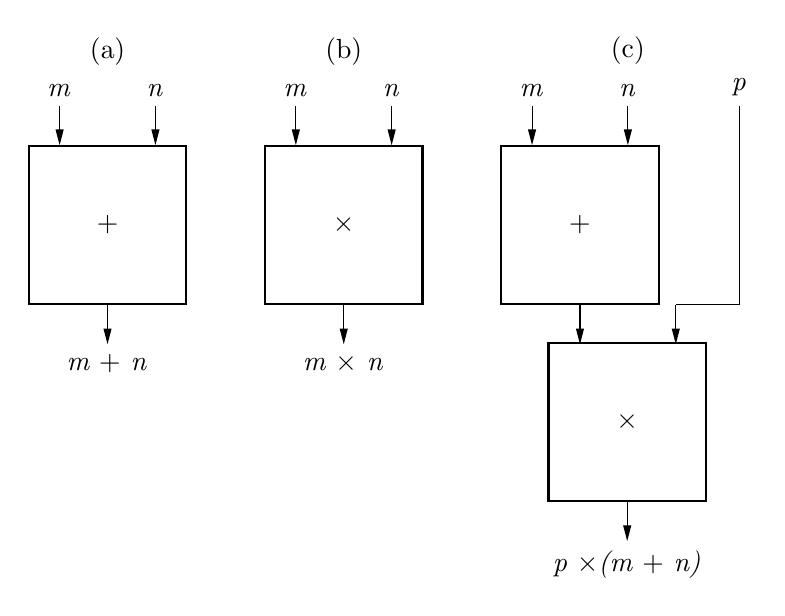
\begin{tikzpicture}
        \foreach \i/\label/\symbol in {0/a/+, 1/b/\times, 2/c/+} {
            \node[draw, minimum size=2cm, thick] (\i) at (\i*3cm,0) {$\symbol$};

            \path (\i.north west) -- (\i.north east)
            coordinate[pos=0.8] (n\i)
            coordinate[pos=0.2] (m\i);

            \draw[{Triangle[length=2mm, width=1mm]}-] (m\i) -- +(0, 0.5cm) node[above] {\textit{m}};
            \draw[{Triangle[length=2mm, width=1mm]}-] (n\i) -- +(0, 0.5cm) node[above] {\textit{n}};

            \ifnum \i=2
                \node (\label) at ($(n\i) + (0, 1.2)$) {(\label)};
    
                \path (\i.north west) -- (\i.north east)
                coordinate[pos=1.5] (p1);
                \path (\i.south west) -- (\i.south east)
                coordinate[pos=1.5] (p2)
                coordinate[pos=1.1] (p3);

                \draw[-] (p1) + (0, 0.5cm) node[above] {\textit{p}} -- (p2);
                \draw[-] (p2) -- (p3);
                \draw[-{Triangle[length=2mm, width=1mm]}] (p3) -- +(0, -0.5cm);
                \draw[-{Triangle[length=2mm, width=1mm]}] (\i.south) -- +(0, -0.5cm);

                \node[draw, minimum size=2cm, thick] (4) at (\i * 3cm + 0.6cm, -2.5cm) {$\times$};
                \draw[-{Triangle[length=2mm, width=1mm]}] (4.south) -- +(0, -0.5cm) node[below] {\textit{p $\times $(m $+$ n)}};
                
            \else
                \node (\label) at (\i*3cm, 2.2) {(\label)};
                \draw[-{Triangle[length=2mm, width=1mm]}] (\i.south) -- +(0, -0.5cm) node[below] {\textit{m $\symbol$ n}};
            \fi
        }
    \end{tikzpicture}
    }
\end{center}

\pagebreak

\section{}
Are items $a$ through $e$ in the following list of algorithms? If not, what qualities required of algorithms do they lack?
\begin{enumerate}[leftmargin=*, label=\textit{\alph*}.]
    \item Add the first row of the following matrix to another row whose first column contains a nonzero entry. (\textit{Reminder}: Columns run vertically; rows run horizontally.)
          \[
              \begin{bmatrix}
                  1  & 2 & 0  & 4  \\
                  0  & 3 & 2  & 4  \\
                  2  & 3 & 10 & 22 \\
                  12 & 4 & 3  & 4
              \end{bmatrix}
          \]
\end{enumerate}

\section{}
Fill in the following truth table for a one-bit AND operation.
\renewcommand{\arraystretch}{1.2}
\begin{center}
    \begin{tabular}{  c  c  | c }
        \hline
        X & Y & X AND Y \\
        \hline
        0 & 0           \\
        0 & 1           \\
        1 & 0           \\
        1 & 1           \\
        \hline
    \end{tabular}
\end{center}

\end{document}

